% Template de rapport de stage scientifique par AT016
% Lire le fichier au fur et à mesure et remplacer par vos valeurs à vous :)
% Au fait ceci est un commentaire

\documentclass[twoside,11pt,openany,a4paper]{rapport}

\graphicspath{{images/}}

\begin{document}

% Non affiché mais sera inséré dans les propriétés du fichier
\title{Complexité du problème de régulation des systèmes de vélo en libre-service sur un ring}
\author{Etienne de \textsc{Saint Germain}}
\date{\today}

\mainmatter

% Page de garde
\begin{titlepage}
  \begin{center}
    
\includegraphics[scale=0.5]{logo_enpc.jpg}
    
    \vspace{0.3cm}
    \institute{École des Ponts ParisTech}\\
    \institute{CERMICS}
    
    \vspace{0.7cm}
    2014\\
    Rapport de stage scientifique
    
    \vspace{0.3cm}
    Etienne \textsc{Gaillard} de \textsc{Saint Germain}\\
    Élève ingénieur\\
    Département IMI
    
    \vspace{2cm}
    {\Huge{\textbf{Complexité du problème de régulation des systèmes de vélo en libre-service sur un ring}}}
    
    \vfill
    {\huge{Stage réalisé au sein du CERMICS}}\\
    École des Ponts ParisTech\\
    6 et 8 avenue Blaise Pascal\\
    Cité Descartes - Champs sur Marne\\
    77455 Marne la Vallée Cedex 2\\

    \vspace{0.7cm}
    Stage effectué du 2 juin au 22 août 2014
    
    \vspace{0.3cm}
    Maître de stage: M. Frédéric Meunier

  \end{center}
\end{titlepage}


\cleardoublepage

\chapter*{Fiche de Synthèse}
\addcontentsline{toc}{chapter}{Fiche de Synthèse}

\begin{itemize}
\item Type de stage : stage scientifique

\item Année académique : 2013/2014

\item Auteur : Etienne \textsc{Gaillard} de \textsc{Saint Germain}

\item Formation : 2ème année

\item Titre du rapport : Complexité du problème de régulation des systèmes de vélo en libre-service sur un ring

\item Organisme d’accueil : CERMICS

\item Pays d’accueil : France

\item Maître de stage : M. Frédéric Meunier

\item Mots-clés caractérisant votre rapport : mathématiques théoriques, compléxité, graphe, optimisation, équilibrage

\item Thème École : Mathématiques
\end{itemize}



\chapter*{Remerciements}
\addcontentsline{toc}{chapter}{Remerciements}


\chapter*{Résumé - Abstract}
\addcontentsline{toc}{chapter}{Résumé - Abstract}

\section*{Résumé}

\textbf{Mots clés :} mathématiques théoriques, complexité, optimisation, graphe, équilibrage
\\

Ce travail s'intéresse au problème du voyageur de commerce avec capacité. Il fait suite à un premier article de P. Benchimol et al. s'intéressant au rééquilibrage d'un graphe et à sa complexité. Le cas du graphe quelconque étant NP-difficile et le cas d'un arbre étant polynomial, nous travaillerons sur le cas du graphe circulaire. Quelques résultats généraux dans le cas général des des graphes circulaires seront démontrés ainsi qu'une solution dans le cas triangulaire et qu'une solution polynomiale dans le cas d'une capacité de transport infinie. Enfin, un cas particulier de la capacité unitaire sera polynomial si une conjecture nécessaire à la démonstration est démontrée dans des travaux ultérieurs.
\\[1cm]

\section*{Abstract}

\textbf{Keywords :}


\tableofcontents
\addcontentsline{toc}{chapter}{Table des matières}
\listoffigures
\addcontentsline{toc}{chapter}{Liste des figures}

\chapter*{Organisme d'accueil : le CERMICS}
\addcontentsline{toc}{chapter}{Organisme d'accueil : le CERMICS}

Le CERMICS (Centre d'Enseignement et de Recherche en Mathématiques et Calcul Scientifique) est un laboratoire de mathématiques appliquées de l'\'Ecole des Ponts ParisTech et de l'Université Paris-Est. Ses activités sont regroupées en trois grands domaines : le calcul scientifique, l'optimisation et les probabilités appliquées.

L'équipe de cacul scientifique s'intéresse aux applications liées à la convection des polluants dans le sol et à l'hydrologie (souterraine ou de surface). Dans ce cadre, elle développe des méthodes numériques basées sur les éléments finis. En plus de ces applications, elle explore une grande variété de sujets liés à la modélisation et à la simulation numérique des phénomènes physiques telle la physique particulaire et multi-échelle. L'étude est à la fois théorique (sur les propriétés des models) et pratique (sur l'implémentation algorithmique).

L'équipe d'optimisation étudie le contrôle des systèmes dynamiques et en particulier les méthodes d'optimisation numérique et stochastique. Elle étudie également les transports ou la gestion de ressources. Enfin, une partie est consacrée à la recherche opérationnelle sous la direction de Frédéric Meunier mon maître de stage. Ici, il s'agit de modéliser des problèmes industriels et d'y apporter des réponses théoriques et pratiques. La recherche peut également se faire sur des questions théoriques encore ouverte dans la recherche opérationnelle.

Pour terminer, en probabilités appliquées sont étudiées les méthodes numériques et probabilistes de représentation des solutions des équations aux dérivées partielles, la modélisation probabiliste de manière générale ou en lien avec la physique, la biologie et les mathématiques financières.


\cleardoublepage

\chapter{Introduction}

\section{Motivations et modèle}

\subsection{Motivations et résultats précédents}
Ce stage s'inscrit dans l'étude des moyens de transport en libre service tel \emph{Vélib'} ou \emph{Autolib'} à Paris. Le principe est le suivant : un utilisateur prend un véhicule dans n'importe quelle station et se déplace jusqu'à une n'importe quelle station où il dépose son véhicule. Un des problèmes auquel est confronté ce service est le taux de foisonnement, c'est-à-dire le fait que chaque station doit garder un bon équilibre entre le nombre de places et le nombre de véhicule. L'étude de ce rééquilibrage sous certaines hypothèse a fait l'objet de recherche et certains résultat ont déjà été publié.
\\

Dans l'article \cite{Benchimol2011}, les auteurs ont introduit une version du \emph{C-delivery TSP}\footnote{littéralement, problème du voyageur de commerce avec livraison et une capacité de transport égale à $C$} défini par Chalasani et Motwani. Le modèle utilisé est nommé \emph{Static Stations Balancing Problem} abrégé SSBP. Ce modèle s'appuie sur un graphe connexe dans lequel un véhicule (que nous appelerons le camion dans la suite) déplace les véhicules en libre service (que nous nommerons vélos) d'un sommet à un autre. Le camion peut transporter un nombre fini et maximal $C$ de vélos, en déposer tout ou une partie à chaque sommet et en prendre dans la limite de sa capacité. L'objectif est de trouver le plus court trajet du camion rééquilibrant le graphe.

Les auteurs ont montré que dans le cas général (capacité $C$ et graphe quelconque), le problème était NP-difficile. Cependant, dans le cas du graphe complet avec des coûts unitaires, ils ont pu obtenir un algorithme donnant une solution au plus deux fois plus coûteuse que la solution optimale.Ils ont également décrit une borne inférieure du coût de la solution optimale\footnote{Cette description et les notations associées seront reprise dans la section \ref{Borne inf générale} afin d'en réutiliser le résultat et le notations.}. Enfin, si le graphe est un arbre, ils ont exhibé un algorithme linéaire donnant le coût d'une solution optimale et le premier mouvement d'une telle solution.
\\

Les auteurs ont également laissé plusieurs questions ouvertes. En particulier, la complexité du rééquilibrage dans le cas où le graphe est un cercle (par exemple des stations le long d'une route entourant un parc) est à ce jour non résolue. Cette question particulière est l'objet de ce stage.

\subsection{Notations et outils}

Soient $F$ un ensemble fini et $H$ un demi-groupe additif. Soit $w \in H^F$. Alors, pour tout sous-ensemble $F'$ de $F$, on note $$w(F') = \sum_{f \in F'} w(f)$$

Soit $G=(V,E)$ un graphe. Pour tout sous-ensemble de sommet $U$ de $V$, on note $\delta(U)$ l'ensemble des arêtes ayant exactement un sommet dans $U$. Par abus de notation, si $v$ est un sommet, on notera $\delta(v)$ au lieu de $\delta(\{v\})$.

Soit $G=(V,E)$ un graphe circulaire. Soit $e \in E$ une arête du graphe. On définit un sens positif dans le graphe. Pour $i \in \ZZ$, on notera $e+i$ la $i^{ème}$ arête $f \in E$ suivant $e$ dans le graphe. (Voir figure \ref{Notation orientation graphe circulaire}.)
\begin{figure}[ht]
  \centering
  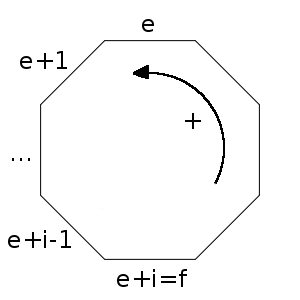
\includegraphics[scale=0.5]{GrapheCirculaire_NotationOrientation.jpg}
  \caption{Orientation du graphe circulaire et ordre des arêtes}
  \label{Notation orientation graphe circulaire}
\end{figure}

Muni d'une telle orientation, pour $u,v \in V$, on définit $\left[ u,v \right]_+$ (resp. $\left[ u,v \right]_-$) l'ensemble des stations rencontrées entre $u$ et $v$ en parcourant $G$ dans le sens positif (resp. négatif). \`A la manière des intervalles, on ouvrira ou fermera les crochets pour exprimer si l'on exclut ou inclut les bornes. (Voir figure \ref{Notation intervalle graphe}.)
\begin{figure}[ht]
  \centering
  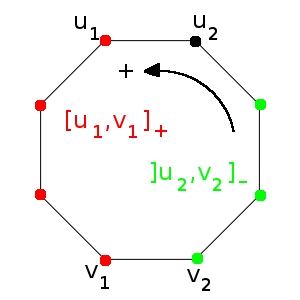
\includegraphics[scale=0.5]{GrapheCirculaire_NotationIntervalle.jpg}
  \caption{Orientation du graphe circulaire et notation sous forme d'intervalle}
  \label{Notation intervalle graphe}
\end{figure}

\subsection{Modèle}

On se donne un graphe $G=(V,E)$ et une capacité $C \ge 0$. Un état $s$ est un couple $(\bs{x},p)$ où $\bs{x} \in \RR^V_+$ et $p$ est une arête dans $V$. Deux états $s=(\bs{x},p)$ et $s'=(\bs{y},q)$ sont dits \emph{adjacents} s'ils ont simultanément :
\begin{itemize}
\item $x_v=y_v$ pour tout $v \notin \{p,q\}$ ;
\item $pq \in E$ ;
\item $x_p-y_p = y_q-x_q$ ;
\item $\left| x_p-y_p \right| \le C$.
\end{itemize}

Un mouvement consiste à aller d'un état $s$ à un état adjacent $s'$. Si le graphe est doté par un coût $\bs{c} \in \RR^E_+$, le coût d'un mouvement entre deux états adjacents $s=(\bs{x},p)$ et $s'=(\bs{y},q)$ est simplement $c(pq)$. Le coût d'une séquence de mouvement est la somme des coût des mouvement de la séquence.
\\

Il est facile de voir que l'état $s=(\bs{x},p)$ code la position $p$ du camion et le nombre $x_v$ de vélos sur chaque stations $v$. Un mouvement correspond bien à un mouvement réel du camion pendant lequel il transorte $x_p-y_p$ vélos de la stations $p$ à la sation $q$.

Dans notre étude, le problème consiste à aller d'un état initial $i=(\bs{x},p)$ à un état final $t=(\bs{y},q)$ en utilisant que des mouvements entre des états adjacents et avec une séquence de coût minimal.

Nous dirons qu'un sommet $v$ (ou une station) est \emph{en excès} (resp. \emph{en défault}) si $x_v > y_v$ (resp. $x_v < y_v$). Une station sera dite \emph{équilibrée} si $x_v=y_v$. L'ensemble des stations équlibrées sera noté $B(\bs{x},\bs{y})$.
\\
La même notion peut être étendue à un sous-ensemble de sommets : $U \subseteq V$ est dit en excès (resp. en défault, équilibré) si $x(U) > y(U)$ (resp. $x(U) < y(U)$, $x(U) = y(U)$).

Pour une séquence de mouvements, pour chaque arête $e \in E$, on notera $z_e$ la variable ``comptant'' le nombre de fois où le camion est passée par l'arête $e$.

Dans l'ensemble de cette étude, nous supposerons également que $x(V) = y(V)$ sinon le problème n'a pas de solutions. En outre, nous supposerons toujours que le graphe possède au moins 3 sommets.
\\

Le problème introduit par les auteurs de l'article \cite{Benchimol2011} s'exprime de la manière qui suit.
\\
\textbf{Données :} Un graphe $G=(V,E)$, une fonction de coût $\bs{c} \in \RR^E_+$, une capacité $C$ et deux états $i=(\bs{x},p)$ (état initial) et $t=(\bs{y},q)$ (état cible).
\\
\textbf{Tâche :} Trouver le coût minimal de la séquence de mouvements permettant d'aller de l'état $i$ à l'état $t$ et le premier mouvement d'une telle séquence.

\section{Résultats}

La section \ref{Résultats préliminaires} présentent les hypothèses de travails et quelques résultats préliminaires sur les graphes circulaires à $n$ sommets. La section \ref{Cas du Triangle} présente un algorithme permettant d'obtenir une solution optimale avec au plus cinq disjonction de cas dans le cas du triangle ainsi qu'une preuve de l'optimalité de la solution retournée par l'agorithme.


\chapter{Résultats préliminaires dans un graphe circulaire à $n$ sommets}
\label{Résultats préliminaires}

\section{Inégalité ``triangulaire'' sur les coûts des arêtes}
\label{sec: Inégalité triangulaire}

On se donne un graphe $G=(V,E)$ circulaire à $n$ sommets et un coût $\bs{c} \in \RR^E_+$. On peut alors faire l'hypothèse suivante :
\begin{gather}\label{Inégalité Triangulaire}
  c_{e'}<\sum_{e \in E \backslash \{e'\}} c_e \quad \text{pour tout } e' \in E
\end{gather}

En effet, supposons qu'il existe $e' \in E$ tel que $c_{e'} \ge \sum_{e \in E \backslash \{e'\}} c_e$.

On se donne une solution optimale $(z_e)_{e \in E}$. Le coût d'une telle solution s'écrit $\Gamma_{G}~=~\sum_{e \in E}~c_ez_e$. On construit alors la séquence de mouvement $(z'_e)_{e \in E}$ par le procédé suivant : chaque passage par l'arête $e'$ est remplacé par un passage sur les autres arêtes avec le même nombre de vélos. Autrement dit, ``on fait le tour dans l'autre sens''. On note $\Gamma'$ le coût d'une telle séquence. On a alors :
\begin{align*}
  \Gamma' &= \sum_{e \in E \backslash \{e'\}} c_e (z_e + z_{e'}) = \sum_{e \in E \backslash \{e'\}} c_ez_e + \left(\sum_{e \in E \backslash \{e'\}} c_{e}\right)z_{e'} \\
     &\le \sum_{e \in E \backslash \{e'\}} c_ez_e + c_{e'}z_{e'} = \Gamma_{G}
\end{align*}

Par conséquent, il existe une solution au moins aussi bonne ne passant pas par $e'$. Pour obtenir la solution optimale, il suffit alors de résoudre le cas du graphe linéaire sur le graphe $G'$ obtenu en supprimant l'arête $e'$ du graphe $G$.

\section{Borne inférieure de la solution optimale (valable pour un graphe quelconque)}
\label{Borne inf générale}

Nous nous contentons ici de récrire la borne inférieure trouvée par les auteurs de l'article \cite{Benchimol2011}.
\\

Une borne inféieure du SSBP est la solution optimale du programme linéaire en nombres entiers dont les variables ``comptent'' le nombre de fois où le camion passe par chaque arête. Les contraintes sont les suivantes :
\begin{enumerate}[label=(\roman*)]
\item les variables sont des entiers naturels.
\item la condition d'Euler : sauf peut-être en $p$ et en $q$, le camion entre et sort de tout sommet un nombre paire de fois.
\item ``subtour elimination'' : si le camion est en $p \in U \subseteq V $ et qu'il existe des stations non-équilibrée dans $\overline{U}$, alors le camion doit nécessairement traverser $\delta(U)$ au moins une fois (voire plus, suivant la position de $q$). Nous utiliserons la notation suivante pour écrire cette contrainte :
\[
\mu(p,q,U,\bs{x},\bs{y}) = \left\{
\begin{array}{ll}
  0 &\mbox{ si } p,q \in U            \mbox{ et } \overline{U} \subseteq B(\bs{x},\bs{y})\\
  0 &\mbox{ si } p,q \in \overline{U} \mbox{ et } U \subseteq B(\bs{x},\bs{y})\\
  1 &\mbox{ si } p \in U              \mbox{ et } q \in \overline{U}\\
  1 &\mbox{ si } p \in \overline{U}   \mbox{ et } q \in U\\
  2 &\mbox{ si } p,q \in U            \mbox{ et } \overline{U} \backslash B(\bs{x},\bs{y}) \ne \emptyset\\
  2 &\mbox{ si } p,q \in \overline{U} \mbox{ et } U \backslash B(\bs{x},\bs{y}) \ne \emptyset
\end{array}
\right.
\]
\item Contrainte de capacité : si $U \subseteq V$ a trop de vélos, le camion doit quitter suffisament de fois $U$ afin de sortir tous ces vélo. Une notation utile est la suivante :
\[
\eta(p,q,U) = \left\{
\begin{array}{ll}
  -1 &\mbox{ si } p \in U            \mbox{ et } q \in \overline{U}\\
  0  &\mbox{ si } p \in U            \mbox{ et } q \in U\\
  0  &\mbox{ si } p \in \overline{U} \mbox{ et } q \in \overline{U}\\
  +1 &\mbox{ si } p \in \overline{U} \mbox{ et } q \in U\\
\end{array}
\right.
\]
\end{enumerate}

Cette borne inférieure est donc solution du programme mathématique en nombres entiers
\begin{gather}\label{PLNE borne inf}
\begin{array}{llll}
  \mbox{Min}_{\bs{z}} &\sum_{e \in E} c_ez_e & & \\
  \mbox{s.c.}       &z_e \in \ZZ_+ &\mbox{pour tout } e \in E &\mbox{(i)} \\
                    &z(\delta(v)) \mbox{ est paire} &\mbox{pour tout } v \in V \backslash \{p,q\}&\mbox{(ii)} \\
                    &z(\delta(U)) \ge \mu(p,q,U,\bs{x},\bs{y}) &\mbox{pour tout } U \subseteq V, U \ne \emptyset &\mbox{(iii)} \\
                    &z(\delta(U)) \ge 2 \left\lceil \frac{x(U)-y(U)}{C} \right\rceil\ + \eta(p,q,U) &\mbox{pour tout } U \subseteq V, U \ne \emptyset &\mbox{(iv)}
\end{array}
\end{gather}

\section{Un exemple où la borne inférieure n'est pas atteinte}

\begin{figure}[ht]
  \label{Exemple de borne inf non atteinte}
  \center 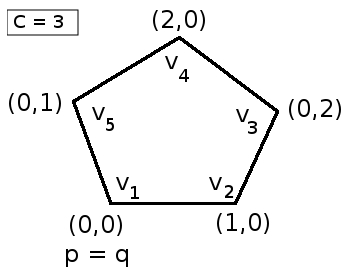
\includegraphics[scale=0.5]{BorneInfNonAtteinte-5sommets.jpg}
  \caption{Exemple de graphe circulaire à 5 sommets où la borne inférieure n'est pas atteinte}
\end{figure}

La solution du programme linéaire en nombre entier \eqref{PLNE borne inf} est $z_e = 1$, pour tout $e \in E$. C'est-à-dire qu'il suffirait de faire un tour complet du graphe sans revenir sur ses pas pour l'équilibrer. Or on constate qu'un tel parcours ne peut pas équilibrer le graphe.

Si dans certains cas particuliers du graphe circulaire, on peut utiliser l'égalité avec la borne inférieure solution du programme mathématique \eqref{PLNE borne inf}, on sait que dans le cas général cette méthode n'aboutira pas. En effet, on vient de montrer qu'il existe des cas où cette borne inférieure n'est pas atteinte.

\section{Changement de variables}
\label{Changement variables}

La description de la borne inférieure dans la section \ref{Borne inf générale} donne un minorant de $z(\delta(U))$ pour toute coupe $\delta(U)$ dans le graphe. Dans le cas de l'arbre décrit dans l'article \cite{Benchimol2011}, on avait donc un minorant de $z_e$ pour tout $e \in E$. Comme $c_e$ est positif pour tout $e\in E$, il suffisait de montrer que le minimum de $z_e$ était atteint pour tout $e \in E$ pour montrer que le coût $\sum_{e _in E}c_ez_e$ était minimal.

\begin{prop}\label{Parité coupe}
Soit $G=(V,E)$ un graphe dont tous les sommets sont de degrès paire. Alors toute coupe de G est de cardinal paire.
\end{prop}

\begin{proof}
Soit $U \subseteq V$. On note $E[U]$ l'ensemble des arêtes de $E$ ayant leur deux sommets dans $U$.
$$
\sum_{v \in U} deg(v) = \sum_{e \in E}\Indic_{\delta(U)}(e)  + 2 \sum_{e \in E}\Indic_{E[U]}(e)
$$
Comme $\sum_{v \in U} deg(v)$ et $2 \sum_{e \in E}\Indic_{E[U]}(e)$ sont paires, on en déduit que le cardinal $\sum_{e \in E}\Indic_{\delta(U)}(e)$ d'une coupe est paire.
\end{proof}

Dans le cas d'un graphe circulaire, tous les sommets sont de degrés deux. Par conséquent, selon la proposition \ref{Parité coupe}, les bornes inférieures des variables $(z_e)_{e \in E}$ ne sont connues que pour des ensembles paires d'arêtes. En supposant connue la valeur de $z(\delta(U))$ pour tout $U \subseteq V$, peut-on retrouver la valeur de $z_e$ pour tout $e \in E$ ?

\begin{lem}\label{Changement de base}
Soit $G=(V,E)$ un graphe circulaire à $n$ sommets ($n \ge 3$). On considère le système linéaire suivant d'inconnues $(z_e)_{e \in E}$ :
\begin{gather}\label{Système linéaire complet}
  \sum_{e \in \delta(U)}z_e = z(\delta(U)) \quad \mbox{pour tout } U \subseteq V \mbox{ tel que } U \ne \emptyset
\end{gather}
On suppose que le système \ref{Système linéaire complet} possède au moins une solution.

Alors cette solution est unique.
\end{lem}

\begin{proof}
La preuve de ce lemme est constructive. On numérote arbitrairement les arêtes du graphe. Il suffit d'extraire le sous-système suivant où chaque colonne représente une arête et où chaque ligne un choix de deux arêtes parmi les $n$ (ie. une coupe) :
\begin{gather}\label{Système linéaire extrait}
  \left(
  \begin{array}{cccccc}
    1 & 0   & 1 & 0      & \cdots & 0 \\
    1 & 1   &   &        &        &   \\
      & 1   & 1 &        & (0)    &   \\
      &     & 1 & 1      &        &   \\
      & (0) &   & \ddots & \ddots &   \\
      &     &   &        & 1      & 1
  \end{array} \right)
  \left(
  \begin{array}{c}
    z_1 \\
    z_2 \\
    z_3 \\
    z_4 \\
    \vdots \\
    z_n
  \end{array} \right)
  =
  \left(
  \begin{array}{c}
    \zeta_1 \\
    \zeta_2 \\
    \zeta_3 \\
    \zeta_4 \\
    \vdots  \\
    \zeta_n
  \end{array} \right)
\end{gather}

On note $M_n$ la matrice du sytème \eqref{Système linéaire extrait}. En développant par rapport à la première ligne, on obtient :
\begin{gather*}
  \mbox{det }M_n =
  1 \times \mbox{det } \left(
  \begin{array}{ccccc}
    1 &                                         &        &        &   \\
    1 & \ddots                                  &        & (0)    &   \\
      & \ddots                                  & \ddots &        &   \\
    \multicolumn{2}{c}{\multirow{2}{*}{ (0) }}  & \ddots & \ddots &   \\
    \multicolumn{2}{c}{}                        &        & 1      & 1
  \end{array} \right)
  + 1 \times \mbox{det } \left(
  \begin{array}{cc|cccc}
    1 & 0                                       & \multicolumn{4}{c}{\multirow{2}{*}{ (0) }} \\
    1 & 1                                       & \multicolumn{4}{c}{}                       \\
    \hline
    \multicolumn{2}{c|}{\multirow{5}{*}{ (0) }} & 1   &        & \multicolumn{2}{c}{\multirow{2}{*}{ (0) }} \\
    \multicolumn{2}{c|}{}                       & 1   & \ddots & \multicolumn{2}{c}{}                       \\
    \multicolumn{2}{c|}{}                       &     & \ddots & \ddots &                                   \\
    \multicolumn{2}{c|}{}                       & (0) &        & 1      & 1
  \end{array} \right)
  = 2
\end{gather*}
Donc le système \eqref{Système linéaire extrait} possède une unique solution.
\end{proof}

On peut également donner une forme explicite de la solution :
\begin{equation}
  \left\{
  \begin{aligned}\notag
    z_1 &= \frac{1}{2}\left(\zeta_1 + \zeta_2 - \zeta_3\right) \\
    z_p &= (-1)^{p-1} z_1 + \sum_{i=2}^p (-1)^{p-i}\zeta_i \quad , \quad \mbox{pour tout } p \in \{2,..,n\}
  \end{aligned}
  \right.
\end{equation}

On obtient ainsi une nouvelle base $\bs{\zeta} = (\zeta_i)_{i \in \{1,..,n\}}$. Nous verrons tout l'intérêt d'un tel changement de variable dans le cas du triangle (section \ref{Cas du Triangle}) et pour montrer que la solution du programme mathématique \eqref{PLNE borne inf} relâché est entière (section \ref{Section solution entiere}).


\section{Solution entière}
\label{Section solution entiere}

\begin{prop} \label{Solution entière}
Pour $n \ge 5$, la solution du programme mathématique \eqref{PLNE borne inf} relâché (ie. avec $z_e \in \RR$ pour tout $e \in E$) est entière.
\end{prop}

Pour démontrer cette proposition, nous avons besoin du résultat suivant :

\begin{prop} \label{cout union}
Soit $X$ et $Y$ deux ensembles de sommets disjoints. Alors
\[z(\delta(X \cup Y)) = z(\delta(X)) + z(\delta(Y)) - 2 z(E[X:Y])\]
où $E[X:Y]$ désigne l'ensemble des arrêtes ayant un sommet dans $X$ et un sommet dans $Y$.
\end{prop}

\begin{proof}
On partitionne $E$ de la manière suivante :\\
- $E_1$, arêtes ne possédant pas de sommets dans $X$ ou dans $Y$ ;\\
- $E_2$, arêtes possédant exactement un sommet dans $X$ et sans sommets dans $Y$ ;\\
- $E_3$, arêtes sans sommets dans $X$ et possédant exactement un sommet dans $Y$ ;\\
- $E[X:Y]$, arêtes possédant un sommet dans $X$ et un sommet dans $Y$.

Alors :\\
- $z(\delta(X \cup Y)) = z(E_2) + z(E_3)$.\\
- $z(\delta(X)) = z(E_2) + z(E[X:Y])$.\\
- $z(\delta(Y)) = z(E_3) + z(E[X:Y])$.

D'où le résultat.
\end{proof}

\begin{proof}[Démonstration de la proposition \ref{Solution entière}]
\begin{figure}[ht]
  \centering
  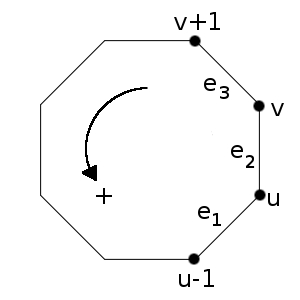
\includegraphics[scale=0.5]{GrapheCirculaire_PreuveSolutionEntiere.jpg}
  \caption{Notations pour la démonstration de la proposition \ref{Solution entière}}
  \label{Numerotation aretes parite}
\end{figure}

On résoud le programme mathématique \eqref{PLNE borne inf} relâché et on note $\bs{z} = (z_e)_{e \in E}$ la solution trouvée. On choisit deux sommets consécutifs $u,v \in U$ tels que $u$ et $v$ soient tout deux différents de $p$ et $q$. Quitte à renuméroter les arêtes, on peut supposer que $e_1 = (u-1,u)$, $e_2 = (u,v)$ et $e_3 = (v,v+1)$. (cf figure \ref{Numerotation aretes parite}.)

Avec les notations introduites dans la section \ref{Changement variables}, on a $\zeta_2~=~z(\delta(u))$ et $\zeta_3~=~z(\delta(v))$ qui sont paires selon la condition d'Euler et $\zeta_1~=~z(\delta({u,v}))$ qui est paire selon la relation de la proposition \ref{cout union}.

\`A l'aide de la forme explicite de la solution du système \eqref{Système linéaire extrait}, on en déduit que $z_1$ est entier, puis par une récurrence immédiate que $z_e$ est entier pour tout $e \in E$.
\end{proof}



\chapter{Cas du triangle}
\label{Cas du Triangle}

\section{Rappel des notations et des hypothèses}

\begin{figure}[ht]
  \label{Notation graphe triangulaire}
  \center 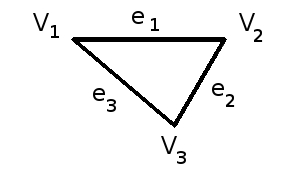
\includegraphics[scale=0.5]{graphe_triangulaire_notations.jpg}
  \caption{Notations utilisées dans le cas du graphe triangulaire}
\end{figure}

Le changement de variables décrit en section \ref{Changement variables} s'écrit ici :
\begin{equation}\notag
  \left\{
    \begin{aligned}
      \zeta_1 &= z_1 + z_3 \\
      \zeta_2 &= z_1 + z_2 \\
      \zeta_3 &= z_2 + z_3
    \end{aligned}
  \right.
  \quad \mbox{et} \quad
  \left(
    \begin{array}{c}
      z_1 \\
      z_2 \\
      z_3
    \end{array}
  \right)
  = \frac{1}{2}
  \left(
    \begin{array}{rrr}
      1 & 1 & -1 \\
      -1 & 1 & 1 \\
      1 & -1 & 1
    \end{array}
  \right)
  \left(
    \begin{array}{c}
      \zeta_1 \\
      \zeta_2 \\
      \zeta_3
    \end{array}
  \right)
\end{equation}
En remplaçant dans la fonction objectif, on obtient :
\begin{equation}\notag
  \sum_{i=1}^3c_iz_i =
    \frac{1}{2} \displayUB{ \left(c_1 - c_2 + c_3 \right) }{>0} \zeta_1
  + \frac{1}{2} \displayUB{ \left(c_1 + c_2 - c_3 \right) }{>0} \zeta_2
  + \frac{1}{2} \displayUB{ \left(-c_1 + c_2 + c_3\right) }{>0} \zeta_3 >0
\end{equation}
Les coefficients des $\zeta_i$ sont positifs à cause de l'hytohèse d'inégalité triangulaire\footnote{cf section \ref{sec: Inégalité triangulaire}}.
\\

Pour un sommet $v \in V$, on définit $U_v$ par $\{v\}$ si $v$ est en excès ou équilibré et par $\overline{\{v\}}$ sinon. On définit également
\[
\zeta_v(p,q,\bs{x},\bs{y}) = \mbox{max} \left( 2 \left\lceil \frac{x(U_v)-y(U_v)}{C} \right\rceil\ + \eta(p,q,U_v), \mu(p,q,U_v,\bs{x},\bs{y}) \right)
\]

\section{Algorithme d'obtention de la solution optimale}

Règles permettant de trouver le premier mouvement d'une solution optimale
\begin{easylist}[articletoc]
& Toutes les stations sont équilibrées.
&& \underline{$p \ne q$}

   Aller de $p$ à $q$.
&& \underline{$p = q$}

   Ne pas bouger (c'est fini).
& Il existe une station non-équlibrée.
&& \underline{$p$ est équilibrée ou en défaut.}

    Aller sur une station en excès sans emporter de vélos.
&& \underline{$p$ est en excès}
&&& \underline{$x(p)-y(p) \ge C$.}

    Prendre C vélos et les déposer sur une station en défaut différente de $q$ si possible, sur $q$ sinon.
&&& \underline{$x(p)-y(p) < C$.}

    Prendre $x(p)-y(p)$ vélos.
&&&& \underline{Les deux autres stations sont en défaut.}

     Déposer les vélos pris sur une station différentes de $q$.
&&&& \underline{Une seule autre station est en défaut.}

     On note $r$ la troisième station en excès ou équilibrée\\
     et $Ex = x(r) - y(r) \pmod{C}$ avec $1 \le Ex \le C$.
&&&&& \underline{$x(p)-y(p)+Ex > C$.}

      Aller sur la station en défaut et déposer les vélos.

&&&&& \underline{$x(p)-y(p)+Ex \le C$.}

      Aller sur la station en excès et déposer les vélos.
\end{easylist}

\begin{thm}
\emph{Optimalité de l'algorithme précédent}

L'algorithme précédent donne le premier mouvement d'une solution optimale et le coût de cette solution est donnée par :
\[
\frac{1}{2} \left(c_1 - c_2 + c_3 \right) \zeta_1(p,q,\bs{x},\bs{y})
+ \frac{1}{2} \left(c_1 + c_2 - c_3 \right) \zeta_2(p,q,\bs{x},\bs{y})
+ \frac{1}{2} \left(-c_1 + c_2 + c_3\right) \zeta_3(p,q,\bs{x},\bs{y})
\]
\end{thm}

\section{Preuve de l'algorithme précédent}

\textbf{$\bs{/!\backslash}$ Il manque un bout à faire \underline{proprement} avec F. Meunier.$\bs{/!\backslash}$}\\ (Si on a la formule de récurrence \ref{Récurrence triangle}, alors, on a bien le résultat de l'algorithme.)

Montrons que :
\begin{gather} \label{Récurrence triangle}
  \zeta_v(p,q,\bs{x},\bs{y}) = \left\{
  \begin{array}{ll}
    1+\zeta_v(p',q,\bs{x'},\bs{y}) & \mbox{si } v=p \mbox{ ou } v=p' \\
    \zeta_v(p',q,\bs{x'},\bs{y}) & \mbox{sinon}
  \end{array}
  \right.
\end{gather}
Dans chacun des différents cas, l'égalité \ref{Récurrence triangle} est évidente dans le cas où $v \ne p$ et où $v \ne p'$.

\subsection*{Cas 1.1 et 1.2}

L'égalité \ref{Récurrence triangle} est évidente dans ce cas.

\subsection*{Cas 2.1}

\begin{minipage}{0.5\linewidth}
\begin{itemize}
\item $p$ équilibré ou en défaut
\item $p'$ en excès
\item on ne transporte pas de vélos
\end{itemize}
\end{minipage}
\begin{minipage}{0.5\linewidth}
\begin{center}
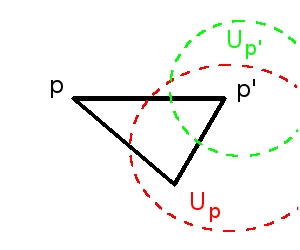
\includegraphics[scale=0.5]{graphe_triangulaire_21.jpg}
\end{center}
\end{minipage}

On note $A = 2 \left\lceil \frac{\displaystyle x(U_p)-y(U_p)}{\displaystyle C} \right\rceil$

\begin{gather*}
  \begin{array}{r|c|c|c|c||c|}
    \multicolumn{2}{c|}{}
    & 2 \left\lceil \frac{x(U_p)-y(U_p)}{C} \right\rceil
    & \eta(p,q,U_p)
    & \mu(p,q,U_p,\bs{x},\bs{y})
    & \zeta_p(p,q,\bs{x},\bs{y})
    \\ \hline
    \multirow{2}{*}{$p$ équilibrée}
    & p=q
    & \multirow{2}{*}{= A = 0}
    & 0
    & 2
    & 2
    \\ \cdashline{2-2}\cdashline{4-6}
    & p \ne q
    &
    & 1
    & 1
    & 1
    \\ \hline
    \multirow{2}{*}{$p$ en défaut}
    & p=q
    & \multirow{2}{*}{$= A \ge 2$}
    & 0
    & 2
    & A
    \\ \cdashline{2-2}\cdashline{4-6}
    & p \ne q
    &
    & 1
    & 1
    & A + 1
    \\ \hline
  \end{array}
\end{gather*}

\begin{gather*}
  \begin{array}{r|c|c|c|c||c|}
    \multicolumn{2}{c|}{}
    & 2 \left\lceil \frac{x'(U_p)-y(U_p)}{C} \right\rceil
    & \eta(p',q,U_p)
    & \mu(p',q,U_p,\bs{x'},\bs{y})
    & \zeta_p(p',q,\bs{x'},\bs{y})
    \\ \hline
    \multirow{2}{*}{$p$ équilibrée}
    & p=q
    & \multirow{2}{*}{= A = 0}
    & -1
    & 1
    & 1
    \\ \cdashline{2-2}\cdashline{4-6}
    & p \ne q
    &
    & 0
    & 0
    & 0
    \\ \hline
    \multirow{2}{*}{$p$ en défaut}
    & p=q
    & \multirow{2}{*}{$= A \ge 2$}
    & -1
    & 1
    & A-1
    \\ \cdashline{2-2}\cdashline{4-6}
    & p \ne q
    &
    & 0
    & 2
    & A
    \\ \hline
  \end{array}
\end{gather*}
Donc $\zeta_p(p,q,\bs{x},\bs{y}) = 1 + \zeta_p(p',q,\bs{x'},\bs{y})$.
\\

On note $B = 2 \left\lceil \frac{\displaystyle x(U_{p'})-y(U_{p'})}{\displaystyle C} \right\rceil$.

\begin{gather*}
  \begin{array}{r|c|c|c||c|}
    & 2 \left\lceil \frac{x(U_{p'})-y(U_{p'})}{C} \right\rceil
    & \eta(p,q,U_{p'})
    & \mu(p,q,U_{p'},\bs{x},\bs{y})
    & \zeta_{p'}(p,q,\bs{x},\bs{y})
    \\ \hline
    p' = q
    & \multirow{2}{*}{$= B \ge 2$}
    & 1
    & 1
    & B + 1
    \\ \cline{1-1}\cline{3-5}
    p' \ne q
    &
    & 0
    & 2
    & B
    \\ \hline
  \end{array}
\end{gather*}

\begin{gather*}
  \begin{array}{r|c|c|c||c|}
    & 2 \left\lceil \frac{x'(U_{p'})-y(U_{p'})}{C} \right\rceil
    & \eta(p',q,U_{p'})
    & \mu(p',q,U_{p'},\bs{x'},\bs{y})
    & \zeta_{p'}(p',q,\bs{x'},\bs{y})
    \\ \hline
    p' = q
    & \multirow{2}{*}{$= B \ge 2$}
    & 0
    & 2
    & B
    \\ \cline{1-1}\cline{3-5}
    p' \ne q
    &
    & -1
    & 1
    & B - 1
    \\ \hline
  \end{array}
\end{gather*}
Donc $\zeta_{p'}(p,q,\bs{x},\bs{y}) = 1 + \zeta_{p'}(p',q,\bs{x'},\bs{y})$.

\subsection*{Cas 2.2.1}

\begin{minipage}{0.5\linewidth}
\begin{itemize}
\item $p$ en excès
\item $p'$ en défaut
\item on transporte $C$ vélos
\item $x(p)-y(p) \ge C$
\end{itemize}
\end{minipage}
\begin{minipage}{0.5\linewidth}
\begin{center}
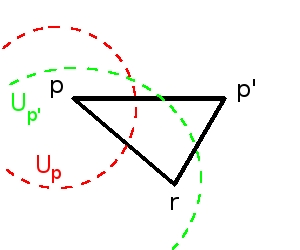
\includegraphics[scale=0.5]{graphe_triangulaire_221.jpg}
\end{center}
\end{minipage}

On note $A = 2 \left\lceil \frac{\displaystyle x(U_p)-y(U_p)}{\displaystyle C} \right\rceil$.

\begin{gather*}
  \begin{array}{c|c|c|c|c||c|}
    \multicolumn{2}{c|}{}
    & 2 \left\lceil \frac{x(U_p)-y(U_p)}{C} \right\rceil
    & \eta(p,q,U_p)
    & \mu(p,q,U_p,\bs{x},\bs{y})
    & \zeta_p(p,q,\bs{x},\bs{y})
    \\ \hline
    p \mbox{ équilibrée}
    & p=q
    & \multirow{2}{*}{$2$}
    & 0
    & 2
    & 2
    \\ \cdashline{2-2}\cdashline{4-6}
    \mbox{après mouvement}
    & p \ne q
    &
    & -1
    & 1
    & 1
    \\ \hline
    p \mbox{ en excès}
    & p=q
    & \multirow{2}{*}{$= A \ge 4$}
    & 0
    & 2
    & A
    \\ \cdashline{2-2}\cdashline{4-6}
    \mbox{après mouvement}
    & p \ne q
    &
    & -1
    & 1
    & A-1
    \\ \hline
  \end{array}
\end{gather*}

\begin{gather*}
  \begin{array}{c|c|c|c|c||c|}
    \multicolumn{2}{c|}{}
    & 2 \left\lceil \frac{x'(U_p)-y(U_p)}{C} \right\rceil
    & \eta(p',q,U_p)
    & \mu(p',q,U_p,\bs{x'},\bs{y})
    & \zeta_p(p',q,\bs{x'},\bs{y})
    \\ \hline
    p \mbox{ équilibrée}
    & p=q
    & \multirow{2}{*}{$0$}
    & 1
    & 1
    & 1
    \\ \cdashline{2-2}\cdashline{4-6}
    \mbox{après mouvement}
    & p \ne q
    &
    & 0
    & 0
    & 0
    \\ \hline
    p \mbox{ en excès}
    & p=q
    & \multirow{2}{*}{$= A-2 \ge 2$}
    & 1
    & 1
    & A-1
    \\ \cdashline{2-2}\cdashline{4-6}
    \mbox{après mouvement}
    & p \ne q
    &
    & 0
    & 2
    & A-2
    \\ \hline
  \end{array}
\end{gather*}
Donc $\zeta_p(p,q,\bs{x},\bs{y}) = 1 + \zeta_p(p',q,\bs{x'},\bs{y})$.
\\

On note $B = 2 \left\lceil \frac{\displaystyle x(U_{p'})-y(U_{p'})}{\displaystyle C} \right\rceil$.

\begin{gather*}
  \begin{array}{r|c|c|c||c|}
    & 2 \left\lceil \frac{x(U_{p'})-y(U_{p'})}{C} \right\rceil
    & \eta(p,q,U_{p'})
    & \mu(p,q,U_{p'},\bs{x},\bs{y})
    & \zeta_{p'}(p,q,\bs{x},\bs{y})
    \\ \hline
    p' = q
    & \multirow{2}{*}{$= B \ge 2$}
    & 1
    & 1
    & B + 1
    \\ \cline{1-1}\cline{3-5}
    p' \ne q
    &
    & 0
    & 2
    & B
    \\ \hline
  \end{array}
\end{gather*}

\underline{$1^{er}$ sous-cas : $p'$ reste en défaut après le mouvement}
\begin{gather*}
  \begin{array}{r|c|c|c||c|}
    & 2 \left\lceil \frac{x'(U_{p'})-y(U_{p'})}{C} \right\rceil
    & \eta(p',q,U_{p'})
    & \mu(p',q,U_{p'},\bs{x'},\bs{y})
    & \zeta_{p'}(p',q,\bs{x'},\bs{y})
    \\ \hline
    p' = q
    & \multirow{2}{*}{$= B \ge 2$}
    & 0
    & 2
    & B
    \\ \cline{1-1}\cline{3-5}
    p' \ne q
    &
    & -1
    & 1
    & B - 1
    \\ \hline
  \end{array}
\end{gather*}

\underline{$2^{ème}$ sous-cas : $p'$ est équlibrée ou en excès après le mouvement}\\
On se place après le mouvement de $p$ à $p'$.
\begin{itemize}
\item \underline{Si $p'=q$}, alors comme $p$ est équilibrée ou en excès, on en déduit que $r$ est équilibrée ou en défaut.\\
Or $r$ n'est pas en défaut (sinon, on serait aller sur $r$ car $p'=q$). Donc $r$ est équilibrée.\\
On en déduit que $p$ et $p'$ sont également équilibrées.\\
D'où : $\zeta_{p'}(p,q,\bs{x},\bs{y}) = 1$ et $\zeta_{p'}(p',q,\bs{x'},\bs{y}) = 0$.

\item \underline{Si $p' \ne q$}
\begin{equation}\notag
\zeta_{p'}(p,q,\bs{x},\bs{y})
= \mbox{max} \left( 2 \left\lceil \frac{x(U_{p'})-y(U_{p'})}{C} \right\rceil + 0, 2\right)
= 2 \left\lceil \frac{ x(U_{p'})-y(U_{p'})}{C} \right\rceil
\end{equation}
\begin{equation}\notag
\zeta_{p'}(p',q,\bs{x'},\bs{y})
= \mbox{max} \left( 2 \left\lceil \frac{x'(U_{p'})-y(U_{p'})}{C} \right\rceil + 1, 1\right)
= 2 \left\lceil \frac{x(U_{p'})-y(U_{p'})}{C} \right\rceil - 1
\end{equation}
\end{itemize}
Dans les deux cas, $\zeta_{p'}(p,q,\bs{x},\bs{y}) = 1 + \zeta_{p'}(p',q,\bs{x'},\bs{y})$.

\subsection*{Cas 2.2.2.1}

\begin{minipage}{0.5\linewidth}
\begin{itemize}
\item $p$ en excès
\item $p'$ et $r$ en défaut
\item $p' \ne q$
\item on transporte $x(p)-y(p)$ vélos
\item $x(p)-y(p) < C$
\end{itemize}
\end{minipage}
\begin{minipage}{0.5\linewidth}
\begin{center}
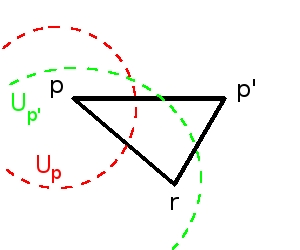
\includegraphics[scale=0.5]{graphe_triangulaire_221.jpg}
\end{center}
\end{minipage}

\begin{gather*}
  \begin{array}{c|c|c|c||c|}
    & 2 \left\lceil \frac{x(U_p)-y(U_p)}{C} \right\rceil
    & \eta(p,q,U_p)
    & \mu(p,q,U_p,\bs{x},\bs{y})
    & \zeta_p(p,q,\bs{x},\bs{y})
    \\ \hline
    p=q
    & \multirow{2}{*}{$2$}
    & 0
    & 2
    & 2
    \\ \cline{1-1}\cline{3-5}
    p \ne q
    &
    & -1
    & 1
    & 1
    \\ \hline
  \end{array}
\end{gather*}

\begin{gather*}
  \begin{array}{c|c|c|c||c|}
    & 2 \left\lceil \frac{x'(U_p)-y(U_p)}{C} \right\rceil
    & \eta(p',q,U_p)
    & \mu(p',q,U_p,\bs{x'},\bs{y})
    & \zeta_p(p',q,\bs{x'},\bs{y})
    \\ \hline
    p=q
    & \multirow{2}{*}{$0$}
    & 1
    & 1
    & 1
    \\ \cline{1-1}\cline{3-5}
    p \ne q
    &
    & 0
    & 0
    & 0
    \\ \hline
  \end{array}
\end{gather*}
Donc $\zeta_p(p,q,\bs{x},\bs{y}) = 1 + \zeta_p(p',q,\bs{x'},\bs{y})$.
\\

\[\zeta_{p'}(p,q,\bs{x},\bs{y}) = \mbox{max}\left(2 \left\lceil \frac{x(U_{p'})-y(U_{p'})}{C} \right\rceil + 0, 2\right)\]
Or $x(U_{p'})-y(U_{p'})<C$ (sinon, $r$ serait en excès).
Donc $\zeta_{p'}(p,q,\bs{x},\bs{y}) = 2$.

\[\zeta_{p'}(p',q,\bs{x'},\bs{y}) = \mbox{max}\left(2 \left\lceil \frac{x'(U_{p'})-y(U_{p'})}{C} \right\rceil + 1,1\right)\]
Or $x(U_{p'})-y(U_{p'})<0$ (car $p$ est équilibrée et $r$ est en défaut).
Donc $\zeta_{p'}(p',q,\bs{x'},\bs{y}) = 1$.
\\
\\
Donc $\zeta_{p'}(p,q,\bs{x},\bs{y}) = 1 + \zeta_{p'}(p',q,\bs{x'},\bs{y})$.

\subsection*{Cas 2.2.2.2.1}

\begin{minipage}{0.5\linewidth}
\begin{itemize}
\item $p$ en excès
\item $p'$ en défaut
\item $r$ en excès ou équilibrée
\item on transporte $x(p)-y(p)$ vélos
\item $x(p)-y(p) < C$
\item $x(p) - y(p) + Ex > C$
\end{itemize}
\end{minipage}
\begin{minipage}{0.5\linewidth}
\begin{center}
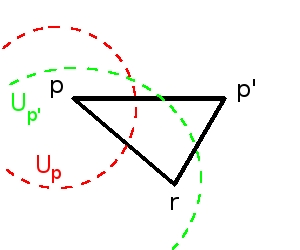
\includegraphics[scale=0.5]{graphe_triangulaire_221.jpg}
\end{center}
\end{minipage}

\begin{gather*}
  \begin{array}{c|c|c|c||c|}
    & 2 \left\lceil \frac{x(U_p)-y(U_p)}{C} \right\rceil
    & \eta(p,q,U_p)
    & \mu(p,q,U_p,\bs{x},\bs{y})
    & \zeta_p(p,q,\bs{x},\bs{y})
    \\ \hline
    p=q
    & \multirow{2}{*}{$2$}
    & 0
    & 2
    & 2
    \\ \cline{1-1}\cline{3-5}
    p \ne q
    &
    & -1
    & 1
    & 1
    \\ \hline
  \end{array}
\end{gather*}

\begin{gather*}
  \begin{array}{c|c|c|c||c|}
    & 2 \left\lceil \frac{x'(U_p)-y(U_p)}{C} \right\rceil
    & \eta(p',q,U_p)
    & \mu(p',q,U_p,\bs{x'},\bs{y})
    & \zeta_p(p',q,\bs{x'},\bs{y})
    \\ \hline
    p=q
    & \multirow{2}{*}{$0$}
    & 1
    & 1
    & 1
    \\ \cline{1-1}\cline{3-5}
    p \ne q
    &
    & 0
    & 0
    & 0
    \\ \hline
  \end{array}
\end{gather*}
Donc $\zeta_p(p,q,\bs{x},\bs{y}) = 1 + \zeta_p(p',q,\bs{x'},\bs{y})$.
\\

On note $\gamma \in \NN \cup \{-1\}$ l'entier tel que $x(r)-y(r)=\gamma. C + Ex$. Alors :
\[
2 \left\lceil \frac{x(U_{p'})-y(U_{p'})}{C} \right\rceil
= 2 \left\lceil \frac{x(p)-y(p)+x(r)-y(r)}{C} \right\rceil
= 2 \left\lceil \frac{x(p)-y(p)+\gamma. C + Ex}{C} \right\rceil
= 2\gamma + 4
\]
\[
2 \left\lceil \frac{x'(U_{p'})-y(U_{p'})}{C} \right\rceil
= 2 \left\lceil \frac{x'(p)-y(p)+x'(r)-y(r)}{C} \right\rceil
= 2 \left\lceil \frac{x(r)-y(r)}{C} \right\rceil
= 2 \left\lceil \frac{\gamma. C + Ex}{C} \right\rceil
= 2\gamma + 2
\]
De plus, $\gamma = -1$ si et seulement si $r$ est équilibrée.

\begin{gather*}
  \begin{array}{c|c|c|c|c||c|}
    \multicolumn{2}{c|}{}
    & 2 \left\lceil \frac{x(U_{p'})-y(U_{p'})}{C} \right\rceil
    & \eta(p,q,U_{p'})
    & \mu(p,q,U_{p'},\bs{x},\bs{y})
    & \zeta_{p'}(p,q,\bs{x},\bs{y})
    \\ \hline
    \multirow{2}{*}{$r$ équilibrée}
    & p'=q
    & \multirow{2}{*}{$2\gamma+4=2$}
    & -1
    & 1
    & 1
    \\ \cdashline{2-2}\cdashline{4-6}
    & p' \ne q
    &
    & 0
    & 2
    & 2
    \\ \hline
    \multirow{2}{*}{$r$ en excès}
    & p'=q
    & \multirow{2}{*}{$2\gamma+4 \ge 4$}
    & -1
    & 1
    & 2\gamma+3
    \\ \cdashline{2-2}\cdashline{4-6}
    & p' \ne q
    &
    & 0
    & 2
    & 2\gamma+4
    \\ \hline
  \end{array}
\end{gather*}

\begin{gather*}
  \begin{array}{c|c|c|c|c||c|}
    \multicolumn{2}{c|}{}
    & 2 \left\lceil \frac{x'(U_{p'})-y(U_{p'})}{C} \right\rceil
    & \eta(p',q,U_{p'})
    & \mu(p',q,U_{p'},\bs{x'},\bs{y})
    & \zeta_{p'}(p',q,\bs{x'},\bs{y})
    \\ \hline
    \multirow{2}{*}{$r$ équilibrée}
    & p'=q
    & \multirow{2}{*}{$2\gamma+2=0$}
    & 0
    & 0
    & 0
    \\ \cdashline{2-2}\cdashline{4-6}
    & p' \ne q
    &
    & 1
    & 1
    & 1
    \\ \hline
    \multirow{2}{*}{$r$ en excès}
    & p'=q
    & \multirow{2}{*}{$2\gamma+2 \ge 2$}
    & 0
    & 2
    & 2\gamma+2
    \\ \cdashline{2-2}\cdashline{4-6}
    & p' \ne q
    &
    & 1
    & 1
    & 2\gamma+3
    \\ \hline
  \end{array}
\end{gather*}
Donc $\zeta_{p'}(p,q,\bs{x},\bs{y}) = 1 + \zeta_{p'}(p',q,\bs{x'},\bs{y})$.

\subsection*{Cas 2.2.2.2.2}

\begin{minipage}{0.5\linewidth}
\begin{itemize}
\item $p$ en excès
\item $p'=r$ en excès
\item la troisième station est en défaut
\item on transporte $x(p)-y(p)$ vélos
\item $x(p)-y(p) < C$
\item $x(p) - y(p) + Ex \le C$
\end{itemize}
\end{minipage}
\begin{minipage}{0.5\linewidth}
\begin{center}
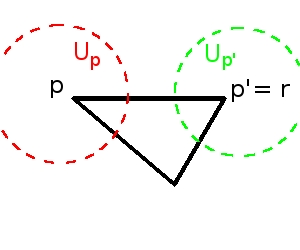
\includegraphics[scale=0.5]{graphe_triangulaire_22222.jpg}
\end{center}
\end{minipage}

\begin{gather*}
  \begin{array}{c|c|c|c||c|}
    & 2 \left\lceil \frac{x(U_p)-y(U_p)}{C} \right\rceil
    & \eta(p,q,U_p)
    & \mu(p,q,U_p,\bs{x},\bs{y})
    & \zeta_p(p,q,\bs{x},\bs{y})
    \\ \hline
    p=q
    & \multirow{2}{*}{$2$}
    & 0
    & 2
    & 2
    \\ \cline{1-1}\cline{3-5}
    p \ne q
    &
    & -1
    & 1
    & 1
    \\ \hline
  \end{array}
\end{gather*}

\begin{gather*}
  \begin{array}{c|c|c|c||c|}
    & 2 \left\lceil \frac{x'(U_p)-y(U_p)}{C} \right\rceil
    & \eta(p',q,U_p)
    & \mu(p',q,U_p,\bs{x'},\bs{y})
    & \zeta_p(p',q,\bs{x'},\bs{y})
    \\ \hline
    p=q
    & \multirow{2}{*}{$0$}
    & 1
    & 1
    & 1
    \\ \cline{1-1}\cline{3-5}
    p \ne q
    &
    & 0
    & 0
    & 0
    \\ \hline
  \end{array}
\end{gather*}
Donc $\zeta_p(p,q,\bs{x},\bs{y}) = 1 + \zeta_p(p',q,\bs{x'},\bs{y})$.
\\

On note $\gamma \in \NN \cup \{-1\}$ l'entier tel que $x(p')-y(p') = x(r)-y(r) = \gamma. C + Ex$. Alors :
\[
2 \left\lceil \frac{x(U_{p'})-y(U_{p'})}{C} \right\rceil
= 2 \left\lceil \frac{x(p')-y(p')}{C} \right\rceil
= 2 \left\lceil \frac{\gamma. C + Ex}{C} \right\rceil
= 2\gamma + 2
\]
\[
2 \left\lceil \frac{x'(U_{p'})-y(U_{p'})}{C} \right\rceil
= 2 \left\lceil \frac{x'(p')-y(p')}{C} \right\rceil
= 2 \left\lceil \frac{x(p)-y(p)+\gamma. C + Ex}{C} \right\rceil
= 2\gamma + 2
\]
De plus, si $\gamma = -1$, alors $p'$ est équilibré ou en défaut, ce qui est faux. Donc $\gamma \ge 0$

\begin{gather*}
  \begin{array}{c|c|c|c||c|}
    & 2 \left\lceil \frac{x(U_{p'})-y(U_{p'})}{C} \right\rceil
    & \eta(p,q,U_{p'})
    & \mu(p,q,U_{p'},\bs{x},\bs{y})
    & \zeta_{p'}(p,q,\bs{x},\bs{y})
    \\ \hline
    p'=q
    & \multirow{2}{*}{$2 \gamma + 2 \ge 2$}
    & 1
    & 1
    & 2 \gamma + 3
    \\ \cline{1-1}\cline{3-5}
    p' \ne q
    &
    & 0
    & 2
    & 2\gamma + 2
    \\ \hline
  \end{array}
\end{gather*}

\begin{gather*}
  \begin{array}{c|c|c|c||c|}
    & 2 \left\lceil \frac{x'(U_{p'})-y(U_{p'})}{C} \right\rceil
    & \eta(p',q,U_{p'})
    & \mu(p',q,U_{p'},\bs{x'},\bs{y})
    & \zeta_{p'}(p',q,\bs{x'},\bs{y})
    \\ \hline
    p'=q
    & \multirow{2}{*}{$2 \gamma + 2 \ge 2$}
    & 0
    & 2
    & 2 \gamma + 2
    \\ \cline{1-1}\cline{3-5}
    p' \ne q
    &
    & -1
    & 1
    & 2\gamma + 1
    \\ \hline
  \end{array}
\end{gather*}
Donc $\zeta_{p'}(p,q,\bs{x},\bs{y}) = 1 + \zeta_{p'}(p',q,\bs{x'},\bs{y})$.
\\

Dans chacun des cas de l'algorithme, l'égalité \ref{Récurrence triangle} est donc vérifiée.


\chapter{Capacité du camion infinie}

Dans tout ce chapitre, on considère un graphe circulaire $G = (V,E)$ à $n$ sommets et muni d'une orientation. On suppose en outre que $p=q$, c'est-à-dire que le point de départ et d'arrivé du camion sont identiques.
\\

Par soucis de concision, nous nommerons ``algorithme dans le cas linéaire'' l'algorithme permettant d'obtenir le premier mouvement de la solution optimale et le coût d'une telle solution dans le cas où le graphe est une ligne. Cet algorithme est décrit dans l'article \cite{Benchimol2011} en section 8. On rappelle qu'un tel algorithme est linéaire en le nombre de sommet.

\section{Algorithme d'obtention de la solution optimale}
\label{Algorithme circulaire infini}

On note $S_{min}$ la meilleure solution réalisable obtenue et on l'initialise avec une solution faisant deux fois le tour du graphe (donc de coût $2\sum_{e \in E}c_e$).

La première partie de l'algorithme va comparer le coût de différentes solutions réalisables sans en calculer le premier mouvement, et une fois la solution optimale $S_{min}$ trouvée, la deuxième partie de l'algorithme donnera les mouvements successifs à faire.
\\

\textbf{Calcul du coût de la solution optimale et de ses caractéristiques :}
\begin{enumerate}
\item\label{Ze0 nul} \uline{Pour chaque $e_o \in E$}
  \begin{enumerate}
  \item Construire le graphe linéaire $\bs{G(e_0)}$ obtenu en supprimant l'arrête $e_0$ de $G$.
  \item Calculer le coût de la solution optimale $S$ à l'aide de l'algorithme dans le cas linéaire.
  \item Si $\Upsilon_{G(e_0)} < \mbox{Coût}(S_{min})$, remplacer les caractéristiques de $S_{min}$ par celles de $S$ (c'est-à-dire son coût et l'arête $e_0$).
  \end{enumerate}
\item\label{Ze0 unitaire} \uline{Pour chaque $w \in V$, pour chaque $w' \in ]w,o]_+$}
  \begin{enumerate}
  \item \uline{Premier cas : sens direct}
    \begin{enumerate}
    \item\label{Ze0 unitaire - direct} Construire le graphe linéaire $\bs{G(w,w',+)}$ obtenu en supprimant les arêtes $E\left[ \left[w',w\right]_+ \right]$ avec :
      \begin{itemize}
      \item $p=w$ et $q=w'$
      \item $x_1(w) = \sum_{v \in E\left[ \left[w',w\right]_+ \right]} x(v)$ et $y_1(w) = 0$
      \item $x_1(w') = 0$ et $y_1(w') = \sum_{v \in E\left[ \left[w',w\right]_+ \right]} y(v)$
      \end{itemize}
    \item Calculer le coût $\Upsilon_{G(w,w',+)}$ de sa solution optimale.
    \item Si $\Upsilon_{G(w,w',+)} + 3 \sum_{ v \in E\left[ \left[w',w\right]_+ \right] }c_v < \mbox{Coût}(S_{min})$, remplacer les caractéristiques de $S_{min}$ par celles de $S$ (c'est-à-dire son coût et le triplet $(w,w',+)$).
    \end{enumerate}
  \item\label{Ze0 unitaire - indirect} \uline{Deuxième cas : sens indirect}
    \begin{enumerate}
    \item Construire le graphe linéaire $\bs{G(w,w',-)}$ obtenu en supprimant les arêtes $E\left[ \left[w',w\right]_+ \right]$ avec :
      \begin{itemize}
      \item $p=w'$ et $q=w$
      \item $x_1(w') = \sum_{v \in E\left[ \left[w',w\right]_+ \right]} x(v)$ et $y_1(w') = 0$
      \item $x_1(w) = 0$ et $y_1(w) = \sum_{v \in E\left[ \left[w',w\right]_+ \right]} y(v)$
      \end{itemize}
    \item Calculer le coût $\Upsilon_{G(w,w',-)}$ de sa solution optimale.
    \item Si $\Upsilon_{G(w,w',-)} + 3 \sum_{ v \in E\left[ \left[w',w\right]_+ \right] }c_v < \mbox{Coût}(S_{min})$, remplacer les caractéristiques de $S_{min}$ par celles de $S$ (c'est-à-dire son coût et le triplet $(w,w',-)$).
    \end{enumerate}
  \end{enumerate}
\end{enumerate}

\textbf{Calcul de la solution optimale :}
\begin{enumerate}
\item\label{Calcul mvt - Ze0 nul} Si $S_{min}$ est caractérisée par une arête $e_0$.
  \begin{enumerate}
  \item Construire le graphe linéaire $\bs{G(e_0)}$.
  \item Calculer les mouvements successifs de la solution optimale à l'aide de l'algorithme dans le cas linéaire sur le graphe $\bs{G(e_0)}$.
  \end{enumerate}
\item\label{Calcul mvt - Ze0 unitaire - direct} Si $S_{min}$ est caractérisée par un triplet $(w,w',+)$.
  \begin{enumerate}
  \item démarrer en $p$.
  \item aller jusqu'à $w'$ dans le sens négatif.
  \item aller jusqu'à $w$ dans le sens positif en ramassant tous les vélos présents sur le chemin.
  \item Construire le graphe linéaire $\bs{G(w,w',+)}$.
  \item Calculer les mouvements successifs de la solution optimale à l'aide de l'algorithme dans le cas linéaire sur le graphe $\bs{G(w,w',+)}$.
  \item aller jusqu'à $w$ dans le sens positif en équilibrant toutes les stations parcourues.
  \item revenir en $p$ dans le sens négatif.
  \end{enumerate}
\item\label{Calcul mvt - Ze0 unitaire - indirect} Si $S_{min}$ est caractérisée par un triplet $(w,w',-)$.
  \begin{enumerate}
  \item démarrer en $p$.
  \item aller jusqu'à $w$ dans le sens positif.
  \item aller jusqu'à $w'$ dans le sens négatif en ramassant tous les vélos présents sur le chemin.
  \item Construire le graphe linéaire $\bs{G(w,w',-)}$.
  \item Calculer les mouvements successifs de la solution optimale à l'aide de l'algorithme dans le cas linéaire sur le graphe $\bs{G(w,w',-)}$.
  \item aller jusqu'à $w'$ dans le sens négatif en équilibrant toutes les stations parcourues.
  \item revenir en $p$ dans le sens positif.
  \end{enumerate}
\end{enumerate}


\begin{thm} \label{thm: optimalité algo infini}
La solution $S_{min}$ retournée à la fin de l'algorithme précédent est une solution réalisable optimale et la complexité de l'algorithme est cubique en le nombre de sommets du graphe.

De plus, le coût de la solution optimale est donnée par
$$
\Upsilon_{G} = \min
\left(
  \min_{e \in E} \Upsilon_{G(e)}\,,\,
  \min_{w \in V, w' \in ]w,o]}
  \left(
    3 \sum_{ v \in E\left[ \left[w',w\right]_+ \right] }c_v + \min \left( \Upsilon_{G(w,w',+)} \,,\, \Upsilon_{G(w,w',-)} \right)
  \right)
\right).
$$
\end{thm}

La suite de ce chapitre va permettre de montrer ce théorème.

\section{Conditions nécessaires pour qu'une solution réalisable soit optimale}

\subsection{Borne supérieure du coût de la solution optimale}

\begin{lem}\label{capacite infinie - borne sup cout}
\emph{Borne supérieure du coût de la solution optimale}\\
Si la capacité $C$ du camion est infine et si $p=q$, alors le coût d'une solution optimale du SSBP est strictement inférieur $\displaystyle 2\sum_{e \in E}c_e$.
\end{lem}

\begin{proof}
Il suffit d'aller de $p$ à $p-1$ dans le sens positif en prenant tous les vélos sur chaque station (y compris en $p$). Tous les vélos du modèle sont alors dans le camion et toutes les stations sont vides. Puis il suffit de revenir de $p-1$ à $p$ dans le sens négatif en posant sur chaque station le nombre de vélo nécessaire pour l'équilibrer.
\end{proof}

En pratique, une capacité infinie signifie que la capacité du camion est supérieure au nombre total de vélos sur le graphe.

\subsection{Parité des $z_e$}

\begin{prop}\label{parité des Ze}
Soit $G=(V,E)$ un graphe connexe. Si $p=q$, alors tous les $z_e$ ont la même parité.
\end{prop}

\begin{proof}
Comme $p=q$, la condition d'Euler est également vérifiée pour $p$. Donc $z(\delta(v))$ est paire pour tout $v \in V$.\\
Soit $e \in E$. Selon la condition d'Euler, $z(\{e, e+1\}) = z_e + z_{e+1}$ est paire. Donc $z_e$ et $z_{e+1}$ ont la même parité. Par une récurrence immédiate, tous les $z_e$ ont la même parité.
\end{proof}

\subsection{Restriction du nombre de passages sur une arête particulière}

\begin{prop}
On suppose que la capacité $C$ du camion est infine et que $p=q$. Soit $S$ une solution optimale du SSBP. Alors il existe une arrête $e_0 \in E$ tel que le camion passe au plus une fois par $e_0$.
\end{prop}

\begin{proof}
Par l'absurde, on suppose que pour tout $e \in E$, le camion passe au moins deux fois sur $e$. Alors le coût de la solution optimale est supérieur à $2\sum_{e \in E}c_e$ ce qui contredit le lemme \ref{capacite infinie - borne sup cout}.
\end{proof}

De cette proposition, on en déduit qu'il suffit de distinguer deux cas :
\begin{itemize}
\item \uline{il existe $e_0 \in E$ tel que le camion ne passe pas par $e_0$.}\\
Dans la partie \ref{Ze0 nul} de l'agorithme, on trouve pour chaque $e_0$ enlevé une solution optimale sous contrainte $z_{e_0} = 0$ et on garde la meilleure.
\item \uline{le camion passe au moins une fois par tous les sommets et il existe $e_0 \in E$ tel que le camion passe exactement une fois par $e_0$.}\\
On démontrera que dans la partie \ref{Ze0 unitaire}, on trouve pour chaque $e_0$ une solution optimale sous contrainte $z_{e_0} = 1$ et on garde la meilleure.
\end{itemize}

\subsection{Restriction du nombre de passages sur l'ensemble des arêtes}

\begin{prop}\label{Ze inf 3 - lineaire}
Soit $G=(V,E)$ un graphe linéaire. On suppose que la capacité $C$ du camion est infine et que $p$ et $q$ sont des extrémités du grapghe. Alors il existe une solution réalisable optimale telle que : pour toute arête $e \in E$, le camion passe au plus trois fois sur $e$.
\end{prop}

\begin{proof}
Les auteurs de l'article \cite{Benchimol2011} ont donné un algorithme et une formule pour calculer les $z_e$ d'une solution optimale particulière. Pour $e \in E$
\begin{gather*}
  z_e = \mbox{max}
  \bigg(
    \underbrace{ 2 \left\lceil \frac{x(U_e)-y(U_e)}{C} \right\rceil\ }_{\displaystyle \le 2 \mbox{ (car } C\mbox{ est infinie)} } +
    \underbrace{ \eta(p,q,U_e) }_{\displaystyle \le 1}\,,\,
    \underbrace{ \mu(p,q,U,\bs{x},\bs{y}) }_{\displaystyle \le 2}
  \bigg)
  \le 3
\end{gather*}
\end{proof}

\begin{lem}\label{Ze inf 3 - circulaire}
Soit $G=(V,E)$ un graphe circulaire. On suppose que la capacité $C$ du camion est infine et que $p=q$. Alors il existe une solution réalisable optimale telle que : pour toute arête $e \in E$, le camion passe au plus trois fois sur $e$.
\end{lem}

\begin{figure}[ht]
  \centering
  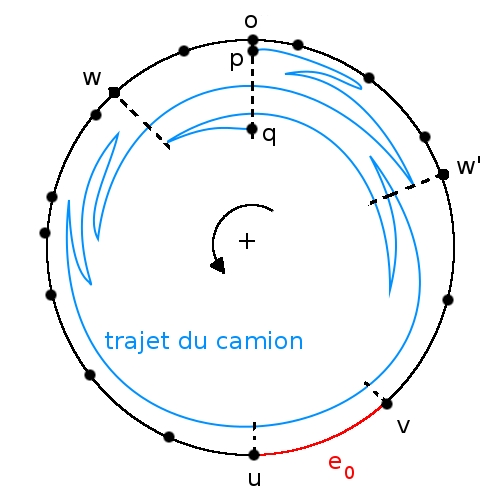
\includegraphics[scale=0.5]{GrapheCirculaire_PreuveZeInf3.jpg}
  \caption{Notations utilisées dans le cas du graphe circulaire avec une capacité infinie}
  \label{Notation graphe circulaire preuve Ze inf 3}
\end{figure}

\begin{proof}\uline{$1^{\mbox{er}}$ cas} : \uline{il existe $e_0 \in E$ tel que le camion ne passe pas par $e_0$.}

Le calcul de la solution optimale se ramène au cas du graphe linéaire $G(e_0)$ obtenu en supprimant l'arête $e_0$ du graphe $G$. Selon la proposition \ref{Ze inf 3 - lineaire}, la solution optimale passe au plus trois fois par chaque arête de $G(e_0)$ donc de $G$.
\\

\uline{$2^{\mbox{ème}}$ cas} : \uline{le camion passe au moins une fois par tous les sommets et il existe $e_0 \in E$ tel que le camion passe exactement une fois par $e_0$.}

Soit $S$ une solution optimale sous contrainte $z_{e_0} = 1$. On note $o=p=q$ le point de départ et d'arrivée du camion. Quitte à changer l'orientation du graphe, on peut supposer que $e_0$ est parcourue dans le sens positif. et on note $u$ le sommet par lequel on entre sur $e_0$ et $v$ le sommet par lequel on sort de $e_0$. (cf figure \ref{Notation graphe circulaire preuve Ze inf 3} pour une synthèse des notations.)

Soit $w$ le sommet sur la portion $[o,u]_+$ le plus proche de $u$ et qui soit atteint par le camion après le parcours de $e_0$. Soit $w'$ le sommet sur la portion $[v,o]_+$ le plus proche de $v$ et qui soit atteint par le camion avant le parcours de $e_0$. Ces deux sommets sont bien définis car $o$ est atteint avant et après le passage sur $e_0$.

Alors, on peut toujours construire une solution optimale $S'$ comme suit :
\begin{enumerate}
\item\label{NewS1} démarrer en $o$.
\item\label{NewS2} aller jusqu'à $w'$ dans le sens négatif.
\item\label{NewS3} aller jusqu'à $w$ dans le sens positif en ramassant tous les vélos présents sur le chemin.
\item\label{NewS4} équilibrer la portion $[w,w']_+$ à l'aide de l'algorithme du cas linéaire sur le graphe $G(w,w',+)$ obtenu à partir de $G$ en supprimant les arêtes $E\left[[w,w']_+\right]$ et tel que :
  \begin{itemize}
  \item $p=w$ et $q=w'$
  \item $\displaystyle x_1(w) = \sum_{v \in E\left[ \left[w',w\right]_+ \right]} x(v)$ et $y_1(w) = 0$
  \item $x_1(w') = 0$ et $\displaystyle y_1(w') = \sum_{v \in E\left[ \left[w',w\right]_+ \right]} y(v)$
  \end{itemize}
\item\label{NewS5} aller jusqu'à $w$ dans le sens positif en équilibrant toutes les stations parcourues.
\item\label{NewS6} revenir en $o$ dans le sens négatif.
\end{enumerate}
Il reste à démontrer que $S'$ équilibre bien le graphe et que $\mbox{Coût}(S') \le \mbox{Coût}(S)$.
\\

\uline{Montrons que $S'$ équilibre bien le graphe.}

\`A l'étape \ref{NewS4}, tous les vélos sont présent dans la portion $[w,w']_+$. La résolution à l'aide de l'algorithme du cas linéaire sur le graphe extrait décrit ci-dessus permet donc d'équilibrer la portion de graphe avec au plus trois passages sur chaque arête de $E\left[[w,w']_+\right]$ (cf Proposition \ref{Ze inf 3 - lineaire}).

\`A la fin de l'étape \ref{NewS4}, les stations de la portion $]w,w'[_+$ sont équilibrées et celles de la portion $[w',w]_+$ sont vides et tous les vélos nécessaires pour l'équilibrer sont sur $w'$. L'étape \ref{NewS5} permet donc bien d'équilibrer les stations de $[w',w]_+$ et l'étape \ref{NewS6} de revenir en $o$.
\\

\uline{Montrons que $\mbox{Coût}(S') \le \mbox{Coût}(S)$.}

Par construction de $w$ et $w'$ la solution $S$ passait au moins trois fois par chaque arête de $[w',w]_+$. Or $S'$ passe exactement trois fois par chaque arête de $[w',w]_+$. Donc $z_e' \le z_e$ pour tout $e \in E\left[ \left[w',w\right]_+\right]$.

On s'intéresse à la solution $S$. On suppose qu'une fois le camion rentré dans $]w,w'[_+$, il retourne dans $[w',w]_+$ en entrant par $w$.\\
- S'il revenait pour prendre des vélos, il aurait pu le faire avant d'entrer dans $]w,w'[_+$.\\
- S'il venait pour poser des vélos, il pourrait le faire après être sorti de $]w,w'[_+$.

On suppose qu'une fois le camion sorti de $]w,w'[_+$, il retourne dans $[w',w]_+$ en entrant par $w'$.\\
- S'il revenait pour prendre des vélos, il aurait pu le faire avant de sortir de $]w,w'[_+$.\\
- S'il venait pour poser des vélos, il aurait pu les prendre avant d'entrer dans $]w,w'[_+$ et les poser une fois à l'intérieur de $]w,w'[_+$.

On en déduit que la solution $S$ équilibre la portion $]w,w'[_+$ comme s'il s'agissait du graphe linéaire $G(w,w',+)$ décrit ci-dessus.
Donc le coût pour équilibrer $]w,w'[_+$ dans $S$ et dans $S'$ est le même.

On en déduit que $\mbox{Coût}(S') \le \mbox{Coût}(S)$ et donc que $S'$ est optimale et réalisable.

Par construction, $S'$ passe au plus trois fois par chaque arête, ce qui conclut la démonstration.
\end{proof}

\section{Preuve de l'optimalité de l'algorithme}

Comme le calcul du coût d'une solution optimale dans le cas d'un graphe linéaire est linéaire en le nombre de sommet, il est évident que l'algorithme décrit en section \ref{Algorithme circulaire infini} est cubique en le nombre de sommet $n$ du graphe $G$.

De plus, il est évident que :
\begin{itemize}
\item $\min_{e \in E} \Upsilon_{G(e)}$ donne le coût de la meilleure solution retourné dans la partie \ref{Calcul mvt - Ze0 nul}.
\item $\min_{w \in V, w' \in ]w,o]} \left(3 \sum_{ v \in E\left[ \left[w',w\right]_+ \right] }c_v + \Upsilon_{G(w,w',+)}\right)$ donne le coût de la meilleure solution retourné dans la partie \ref{Calcul mvt - Ze0 unitaire - direct}.
\item $\min_{w \in V, w' \in ]w,o]} \left(3 \sum_{ v \in E\left[ \left[w',w\right]_+ \right] }c_v + \Upsilon_{G(w,w',-)}\right)$ donne le coût de la meilleure solution retourné dans la partie \ref{Calcul mvt - Ze0 unitaire - indirect}.
\end{itemize}
Donc la formule donnée dans le théorème \ref{thm: optimalité algo infini} donne bien le coût de la meilleure solution retournée par l'algorithme.

Il reste à montrer que l'algorithme renvoie bien une solution optimale.

\chapter{Capacité du camion unitaire}

\chapter{Questions ouvertes}

\chapter*{Bilan personnel}
\addcontentsline{toc}{chapter}{Bilan personnel}

J'ai choisi ce stage en Recherche Opérationnelle afin d'appliquer mes connaissances acquises pendant le cours de deuxième année \emph{Initiation à la Recherche Opérationnelle} et de me préparer à ma deuxième année de master que j'effectuerai au CNAM en suivant le \emph{Master Parisien de Recherche Opérationnelle}. Je suis très satisfait de ce stage qui a répondu à ce double objectif et me conforte dans mon choix de Master 2. J'y ai également appris à persévérer sur un problème ouvert et à discuter des solutions envisagées. Même si la question initiale n'est pas résolue, je suis content des résultats intermédiaires trouvés.

De plus, j'ai pu mieux appréhender ce qu'était la recherche en Recherche Opérationnelle. J'ai beaucoup apprécié pouvoir consacrer beaucoup plus de temps qu'en \'Ecole à la résolution d'un problème. Lors du stage de fin d'étude, je souhaiterais comparer cette expérience avec un travail où il faut apporter une réponse, éventuellement partielle, en temps limité à un problème concret apporté par un acteur industriel.


\bibliographystyle{siam}
\bibliography{rapport}
\addcontentsline{toc}{chapter}{Bibliographie}

\backmatter

\end{document}
